\documentclass[twocolumn]{myarticle}

\usepackage{mymacros}
\usepackage{parskip}
\usepackage{hyperref}
\usepackage{listings}
\usepackage{booktabs}

\lstset{%
basicstyle=\small\ttfamily,
columns=flexible,
breaklines=true,
numbers=left,
stepnumber=1,}

\begin{document}

\title{Monte Carlo methods in computational physics}
\author{Casey Daniel and Chris Deimert}
\date{\today}

\maketitle

\section{Introduction}
\label{sec:introduction}

In this report, we explore a number of Monte Carlo numerical methods.
Monte Carlo methods use pseudorandom numbers to explore complicated systems.
These methods tend to converge slowly for simple problems, but can be very efficient for complex problems: especially those with a large number of variables.

\section{Pseudo random numbers}
\label{sec:pseudo_random_numbers}

Monte Carlo methods typically rely heavily on our ability to generate a large quantity of random numbers.
We cannot, of coure, generate truly random numbers on a deterministic computer, so we have to approximate them with pseudo-random numbers (PRN's).
Having a reliable PRN generator is thus a key prerequisite to any Monte Carlo method.
In this section, we will study the linear congruential method (LCM) for generating PRN's.
The LCM generates a sequence of pseudo-random integers with the $ n $th integer given by
\begin{align}
    I_{n} &= \left( A I_n + C \right) \! \! \! \! \! \mod M
\end{align}
($ I_0 $ is called the "seed".)
We can then generate a sequence $ x_n = I_n/M $ of pseudo-random real numbers with $ 0 < x_n < 1 $.

A Fortran 90 module was created to implement the LCM generator and can be seen in Section~\ref{subsec:pseudo_random_numbers_module}.
This code was tested in a number of ways, the code for which is in Section~\ref{subsec:pseudo_random_numbers_main_code} and Section~\ref{subsec:pseudo_random_numbers_plotting_code}.)

The first, simplest test used $ I_0 = 3 $, $ A = 7 $, $ C = 0 $, and $ M = 10 $.
The result is a repeating sequence of numbers:
\begin{align}
    x &= 0.1, 0.7, 0.9, 0.3, 0.1, 0.7, 0.9, 0.3, \ldots
\end{align}
This sequence repeats after only 4 numbers, demonstrating why small values of $ M $ are a poor choice.
The sequence will repeat after at most $ M $ numbers, so we must select a high value of $ M $ in order to obtain a long sequence (though high values of $ M $ do not \emph{guarantee} a long sequence).

One useful way to test a pseudo-random number generator is to look at the correlation between each generated number and the number that preceded it.
These can be plotted in a 2D scatter plot: patterns on the scatter plot imply that the pseudo-random number generator is actually predictable and thus not very random.
The correlation plots for three different sets of coefficients are shown in Figures \ref{fig:LCM_test_1}, \ref{fig:LCM_test_2}, and \ref{fig:LCM_test_3}.
Note that a seed of $ I_0 = 1 $ was used in each case.
It is found that the third combination of coefficients provides the best pseudo-random number generator.

\begin{figure}[ht!]
    \begin{center}
    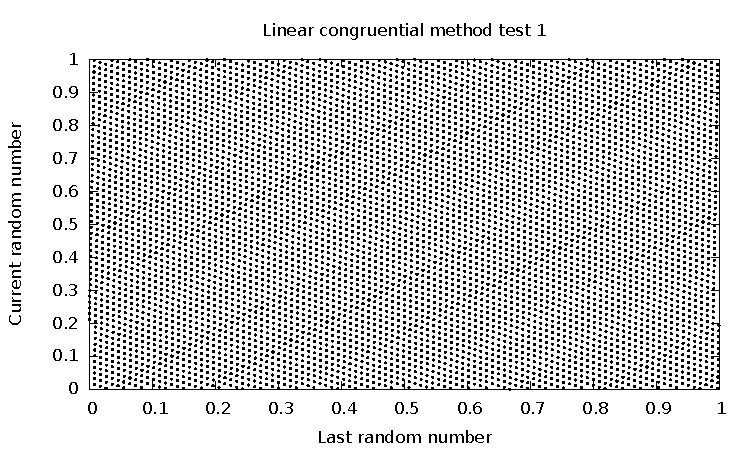
\includegraphics[width = 0.45\textwidth]{../Plots/LCM_test_1.pdf}
    \caption{%
        The correlation plot for $ A = 106 $, $ C = 1283 $, and $ M = 6075 $ is shown below.
        It is seen that the correlation plot is strongly patterned, meaning that this is a relatively predictable sequence of numbers.
        Thus, this choice of LCM coefficients is a poor one.
    }
    \label{fig:LCM_test_1}
    \end{center}
\end{figure}

\begin{figure}[ht!]
    \begin{center}
    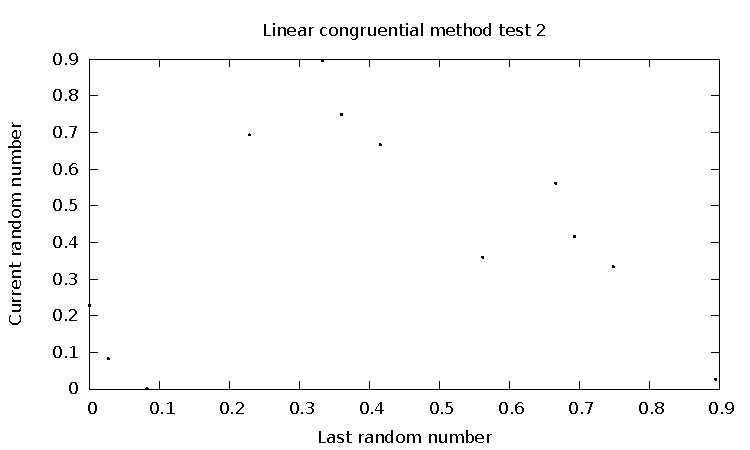
\includegraphics[width = 0.45\textwidth]{../Plots/LCM_test_2.pdf}
    \caption{%
        The correlation plot for $ A = 107 $, $ C = 1283 $, and $ M = 6075 $ is shown below.
        It is seen that the correlation plot is even more strongly patterned than the last one.
        Thus, this is a relatively predictable sequence of numbers and this choice of LCM coefficients is poor.
        This also demonstrates how small changes in the coefficients lead to drastic changes in the effectiveness of the LCM generator.
        (The coefficients here are the same as the last set except that $ A $ has been increased by 1).
    }
    \label{fig:LCM_test_2}
    \end{center}
\end{figure}

\begin{figure}[ht!]
    \begin{center}
    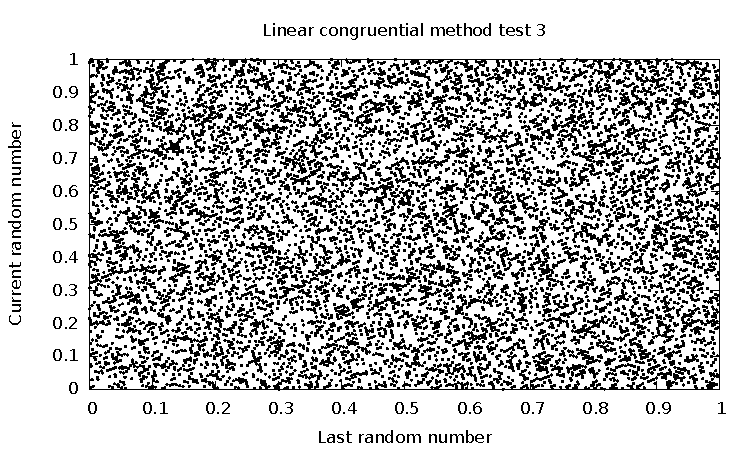
\includegraphics[width = 0.45\textwidth]{../Plots/LCM_test_3.pdf}
    \caption{%
        The correlation plot for $ A = 1103515245 $, $ C = 12345 $, and $ M = 32768 $ is shown below.
        It is seen that the correlation plot is very weakly patterned, meaning that this is a relatively unpredictable sequence of numbers.
        Thus, this choice of LCM coefficients is a good one.
    }
    \label{fig:LCM_test_3}
    \end{center}
\end{figure}

Another test of pseudo-random number generators that can be performed is a $ \chi^2 $ test.
This is used to determine our statistical confidence in the fact that the pseudo-random numbers are evenly generated.

Using the LCM generator with a seed of $ I_0 = 1 $ and coefficients from the third test above, 100 numbers were generated.
Similarly, 100 numbers were generated using the gfortran generator with a seed based on the computer time.
The distribution of results are shown below.

\bigskip
\begin{center}
    \begin{tabular}{ccccc}
        \toprule
        Interval & Upper limit & LCM & gfortran & Exp. \\
        \midrule
        1  & 0.1 &  6 &  6 & 10 \\
        2  & 0.2 & 11 & 16 & 10 \\
        3  & 0.3 & 12 &  9 & 10 \\
        4  & 0.4 &  9 &  6 & 10 \\
        5  & 0.5 & 10 & 11 & 10 \\
        6  & 0.6 &  9 &  5 & 10 \\
        7  & 0.7 &  8 & 12 & 10 \\
        8  & 0.8 & 10 &  9 & 10 \\
        9  & 0.9 & 11 & 13 & 10 \\
        10 & 1.0 & 14 & 13 & 10 \\
        \bottomrule
    \end{tabular}
\end{center}
\bigskip

The $ \chi^2 $ values for the LCM and gfortran generators are:
\begin{align}
    \chi_{\text{LCM}}^2 &= 6.80
    \\
    \chi_{\text{gfortran}}^2 &= 8.40
\end{align}

These were calculated using 
\begin{align}
    \chi^2 &= \sum_{i=1}^{10} \frac{(O_i - E_i)^2}{E_i}
\end{align}
where $ O_i $ is the observed value in the $ i $th row of the table above, and $ E_i $ is the expeced value. 

It should be noted that the $ \chi^2 $ values change significantly depending on the seed used, though the ones given here are fairly typical.
The LCM $ \chi^2 $ varies from about 2 to about 10, and the gfortran $ \chi^2 $ varies from about 3 to about 18.

In this case, our null hypothesis is that the generated random numbers which are independent and uniformly distributed between 0 and 1.
We have 9 degrees of freedom in this case, which means that the critical $ \chi^2 $ value for 95\% confidence is $ \chi_{\text{crit}}^2 = 16.92 $.
Thus we cannot confidently reject the hypothesis that the pseudo-random number generators are uniformly distributed and independent.

It should be noted that if the number of trials is increased from 100, the $ \chi^2 $ for the LCM decreases while the $ \chi^2 $ for the gfortran remains approximately the same.
We would expect the $ \chi^2 $ to decrease for truly random numbers (from the law of large numbers), so this indicates a problem with the gfortran generator.

A final test we can perform is the auto-correlation test for independence.
The autocorrelation $ A_k $ of a sequence of random variables represents the correlation between the $ t $th number and the $ t+k $th random number.
It is given by
\begin{align}
    A_k &= \frac{\displaystyle \sum_{t=1}^{N-k}\big(x_t - \left\langle x \right\rangle\big)\big( x_{t+k} - \left\langle x \right\rangle \big)}{\displaystyle \sum_{t=1}^{N-k} \big( x_t - \left\langle x \right\rangle \big)^2}
\end{align}


\onecolumn

\section{Code}
\label{sec:code}

\subsection{Pseudo random numbers module}
\label{subsec:pseudo_random_numbers_module}

\lstinputlisting[breaklines]{../../Modules/Random_numbers_module.f90}
\vspace{10pt}

\subsection{Pseudo random numbers main code}
\label{subsec:pseudo_random_numbers_main_code}

\lstinputlisting[breaklines]{../Pseudo_RNGs.f90}
\vspace{10pt}

\subsection{Pseudo random numbers plotting code}
\label{subsec:pseudo_random_numbers_plotting_code}

\lstinputlisting[breaklines]{../Pseudo_RNGs.gp}
\vspace{10pt}

\end{document}
